%%
%% Progress check-in (11 Nov 2026) do projeto de PPC.
%% Página 1: introdução, ambiente e método. Página 2: resultados. Página 3: o programa (Java).
%%
\documentclass[sigplan]{acmart}
\settopmatter{printacmref=false}
\renewcommand\footnotetextcopyrightpermission[1]{}
\usepackage{array}
\usepackage{booktabs}
\usepackage[portuguese]{babel}
\usepackage{enumitem}
\setlist{nosep,leftmargin=*}
\usepackage{tikz}
\usetikzlibrary{positioning,fit,backgrounds,arrows.meta,calc,decorations.pathreplacing}
\definecolor{azul}{HTML}{2A78D6}
\definecolor{laranja}{HTML}{EB6834}

\raggedbottom
\setlength{\emergencystretch}{1.5em}
\begin{document}

\title{Check-in: Distribuição de Tarefas Plana vs.\ Hierárquica num Pequeno Cluster Emulado}

\author{Gonçalo Lourenço}
\affiliation{%
 \institution{Programação Paralela e Concorrente, Faculdade de Ciências, Universidade de Lisboa}}
\email{fc68092@alunos.ciencias.ulisboa.pt}

\pagestyle{plain}
\maketitle

% Fica no topo da página 2.
\begin{figure*}[t]
  \centering
  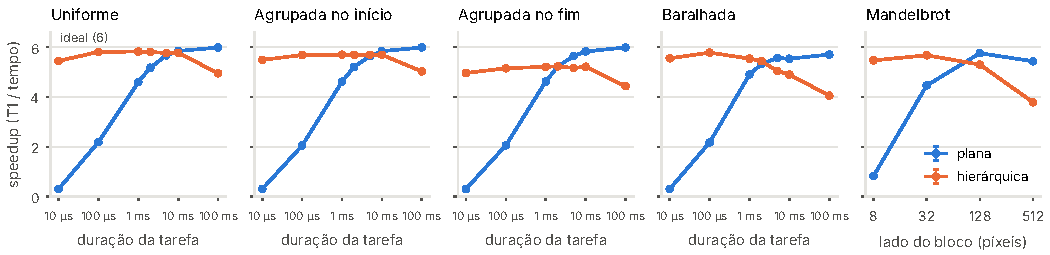
\includegraphics[width=\textwidth]{figuras/paper_grelha}
  \caption{Speedup ($T_1/T_6$): mediana e IC a 95\% (bootstrap; quase sempre menor do que o
  ponto). A carga sintética com cada desequilíbrio e o Mandelbrot; a tracejado, o ideal.}
  \label{fig:grelha}
\end{figure*}

\section{Introdução}

Num sistema mestre--trabalhador distribuído, um coordenador reparte tarefas independentes
por nós ligados em rede. Comparo duas formas de o fazer:
\begin{itemize}
  \item \textbf{plana}: cada thread de cada nó pede ao coordenador uma tarefa de cada vez;
  \item \textbf{hierárquica}: um gestor em cada nó pede um lote de $k$ tarefas e reparte-o
        pelas threads do nó.
\end{itemize}
A plana equilibra melhor a carga, mas paga uma ida e volta na rede por tarefa. A hierárquica
paga uma por lote, mas pode deixar threads paradas quando os lotes custam tempos diferentes.
Meço, num cluster de 3 nós com 2 cores cada, em que tamanhos de tarefa e desequilíbrios de
carga cada uma é mais rápida. Testo três hipóteses:
\begin{itemize}
  \item \textbf{H1}: com tarefas pequenas, a hierárquica é mais rápida;
  \item \textbf{H2}: com tarefas grandes e carga desequilibrada, a plana é mais rápida;
  \item \textbf{H3}: há um ponto de cruzamento, que se desloca para tarefas mais pequenas
        quando o desequilíbrio aumenta.
\end{itemize}
Implementei as duas políticas de raiz em Java 21, sobre TCP (o programa está na Fig.~\ref{fig:diagrama}, na página~3).

\section{Ambiente experimental}

\noindent\textbf{Torre (os 3 nós).}
\begin{itemize}
  \item AMD Ryzen 7 3700X (8 cores), 32\,GB, Ubuntu Server 24.04, kernel 6.8.
  \item 3,6\,GHz fixos; SMT, \emph{boost} e o estado de sono C2 (400\,$\mu$s) desligados.
  \item Cada nó é um contentor Docker 29.9 com uma JVM, preso a 2 cores: nó 1 nos cores
        0--1, nó 2 nos 2--3, nó 3 nos 4--5.
  \item O sistema fica nos cores 6--7 (cgroups).
  \item Java 21 (Temurin), heap fixo de 512\,MB, \emph{Serial GC}.
\end{itemize}

\smallskip
\noindent\textbf{Portátil (o coordenador).}
\begin{itemize}
  \item Intel Core i7-13620H, 16\,GB, kernel 7.0, OpenJDK 21.0.12.
  \item Gera as tarefas, distribui-as, verifica os resultados e grava os dados; não calcula.
  \item Perfil \emph{performance} e sono do CPU limitado a 2\,$\mu$s de latência; Wi-Fi e
        atualizações desligados durante as medições.
  \item Ligado à torre por um switch Gigabit: ida e volta de 120\,$\mu$s (mediana), 941\,Mbit/s.
\end{itemize}

\section{Como medi}

\noindent\textbf{Cargas.} \emph{Sintética}: um ciclo \emph{xorshift64} sobre inteiros, sem
memória, calibrado na torre (1,6755\,ns por iteração). Tarefas de 10\,$\mu$s, 100\,$\mu$s,
1, 2, 5, 10 e 100\,ms, com 2,4\,s de trabalho por repetição (12\,s nos 100\,ms). Quatro
desequilíbrios, todos com o mesmo trabalho total:
\begin{itemize}
  \item \emph{uniforme}: todas as tarefas iguais;
  \item \emph{agrupada no início} e \emph{no fim}: 10\% das tarefas 10$\times$ mais longas,
        seguidas no início ou no fim da fila;
  \item \emph{baralhada}: as mesmas 10\%, em posições aleatórias.
\end{itemize}
\emph{Mandelbrot}: 4096$\times$4096 píxeis, até 1000 iterações, em blocos de lado 8, 32,
128 e 512. O desequilíbrio é natural: medi cada bloco num core e 15 a 22\% dos blocos levam
90\% do tempo.

\smallskip
\noindent\textbf{Repetições.} Corri 50 repetições seguidas em 4 configurações: a maior queda
(JIT) dá-se nas 3 primeiras. Descarto 10 e meço 30 (20 nos 100\,ms). Na grelha não sobra
deriva: entre as primeiras e as últimas 10 repetições medidas, a variação mediana é de $-$0,07\%.

\smallskip
\noindent\textbf{Lote.} Na hierárquica, $k$ = tarefas/24: 24 lotes por repetição, 8 por nó.
Com 20 lotes, um nó ficava com 7 e outro com 6, e a hierárquica nunca passava de 95\% de
eficiência. Varri $k$ de 1 a 10\,000 em 4 tamanhos: a regra fica sempre a menos de 3\% do
melhor lote.

\smallskip
\noindent\textbf{Linha de base.} $T_1$ é a mesma carga com 1 nó de 1 thread, pelo mesmo
caminho (Docker, rede, coordenador); o speedup é $T_1/T_6$. O caminho custa 0,1 a 4,7\% em
relação ao cálculo puro.

\smallskip
\noindent\textbf{Controlo.} As 64 configurações correm por ordem aleatória, numa só sessão de
2 horas. Em cada repetição verifico que cada tarefa chegou uma vez e que o XOR dos resultados
iguala o sequencial. Os 3 pares de cores diferem 0,26\%; a torre não passou de 49\,$^\circ$C.

\smallskip
\noindent\textbf{Estatística.} Só 21 das 64 amostras passam no Shapiro-Wilk, por isso comparo
as políticas com Mann-Whitney U e correção de Holm (32 comparações), e meço o efeito com o
$\delta$ de Cliff e a razão das medianas.

% ------------------------------------------------------------------ página 2
\newpage
\section{Resultados}

\begin{table}[t]
  \caption{Razão das medianas plana/hierárquica ($>1$: a hierárquica é mais rápida).
  $p_{\text{Holm}} < 0{,}01$ em todas, exceto *. $\dagger$: lote ímpar.}
  \label{tab:razao}
  \scriptsize
  \setlength{\tabcolsep}{4pt}
  \begin{tabular}{@{}lrrrr@{}}
    \toprule
    Tarefa & Uniforme & Agr.\ início & Agr.\ fim & Baralhada \\
    \midrule
    10\,$\mu$s  & 17,6  & 17,5  & 15,7  & 17,8 \\
    100\,$\mu$s & 2,65  & 2,77  & 2,50  & 2,65 \\
    1\,ms       & 1,27  & 1,23  & 1,13  & 1,13 \\
    2\,ms       & 1,12  & 1,09  & 1,00* & 1,02 \\
    5\,ms       & 1,02  & 1,01  & 0,92  & 0,91 \\
    10\,ms      & 0,99  & 0,98  & 0,90  & 0,89 \\
    100\,ms     & 0,83$\dagger$ & 0,84$\dagger$ & 0,74$\dagger$ & 0,71$\dagger$ \\
    \midrule
    \multicolumn{5}{@{}l}{Mandelbrot, lado 8 / 32 / 128 / 512: \;6,58 / 1,27 / 0,92 / 0,70$\dagger$} \\
    \bottomrule
  \end{tabular}
\end{table}

\noindent\textbf{H1: confirmada} (Fig.~\ref{fig:grelha}, Tab.~\ref{tab:razao}). Com 10\,$\mu$s,
a hierárquica é 15,7 a 17,8$\times$ mais rápida; com 1\,ms, ainda 1,13 a 1,27$\times$. A causa
é o número de mensagens: com 10\,$\mu$s, a plana troca 720\,000 por repetição e a hierárquica
72, para um volume parecido (4,0 vs.\ 2,8\,MB). As threads da plana passam 95\% do tempo à
espera (Fig.~\ref{fig:parado}).

\smallskip
\noindent\textbf{H2: confirmada.} Com 5 e 10\,ms e as longas no fim ou baralhadas, a plana é
1,09 a 1,13$\times$ mais rápida ($\delta = -1$); no Mandelbrot de lado 128, 1,09$\times$. O
mecanismo vê-se na Fig.~\ref{fig:parado}: com as longas no fim, os 2 últimos lotes são
pesados e prendem 2 nós, enquanto o terceiro fica 34\% do tempo parado. A plana reparte essas
tarefas uma a uma e mantém as 6 threads a 97\%. Com as longas \emph{no início}, os lotes
pesados saem primeiro e os leves preenchem o fim: as duas políticas quase empatam.

\begin{figure}[t]
  \centering
  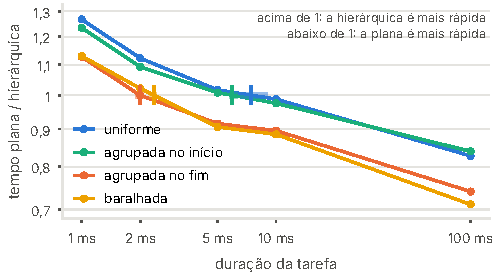
\includegraphics[width=\columnwidth]{figuras/paper_cruzamento}
  \caption{Razão plana/hierárquica entre 1 e 100\,ms. Traço: o cruzamento (interpolado em
  log-log); barra: o seu IC a 95\% (bootstrap).}
  \label{fig:cruzamento}
\end{figure}

\begin{figure}[t]
  \centering
  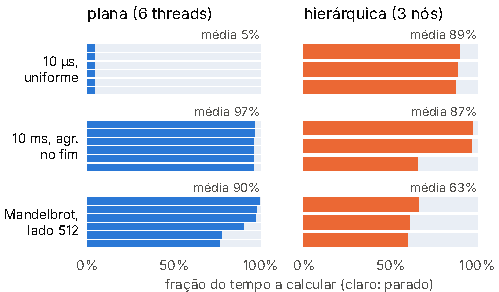
\includegraphics[width=0.9\columnwidth]{figuras/paper_parado}
  \caption{Fração do tempo a calcular, por thread (plana) ou por nó (hierárquica), da mais à
  menos ocupada.}
  \label{fig:parado}
\end{figure}

\smallskip
\noindent\textbf{H3: confirmada} (Fig.~\ref{fig:cruzamento}). O cruzamento fica nos 7,5\,ms
com a carga uniforme [IC 6,6--9,1], e desce para 5,9\,ms com as longas no início [5,7--6,4],
2,4\,ms com as baralhadas [2,2--2,4] e 2,0\,ms com as longas no fim [1,9--2,1]. Os ICs dos
três desequilíbrios não tocam no da uniforme.

\smallskip
\noindent\textbf{Lote ímpar ($\dagger$).} Nos 100\,ms, o lote de 5 tarefas para 2 threads
deixa uma thread parada no fim de cada lote: 83\% de eficiência mesmo na uniforme (o mecanismo
da H2, isolado). O efeito é igual nos 4 desequilíbrios, por isso comparo-os entre si: face à
uniforme, a hierárquica fica 1,12$\times$ mais lenta com as longas no fim e 1,22$\times$ com as
baralhadas. O lado 512 tem o mesmo efeito (lote de 3).

\smallskip
\noindent\textbf{Ameaças.} Os nós partilham a cache L3; o JIT varia 1--2\% entre arranques
da JVM. \textbf{Próximo passo.} Política hierárquica com \emph{work stealing} entre nós,
medida na mesma grelha.

\smallskip
\noindent\textbf{Uso de IA.} Usei o Claude (Anthropic) no apoio ao código, nos scripts de
execução e de análise e na redação.

% ------------------------------------------------------------------ página 3
\clearpage
\begin{figure*}[p]
  \centering
  \resizebox{0.93\textwidth}{!}{% Página 3: como o programa funciona (Java). Duas partes:
%   (a) componentes, threads e objetos partilhados, no coordenador e no nó, e o protocolo;
%   (b) uma repetição, passo a passo, na plana e na hierárquica.
\begin{tikzpicture}[
    font=\scriptsize, >=Stealth,
    thr/.style={draw=laranja, fill=laranja!9, rounded corners=2pt, align=left, inner sep=3pt,
                anchor=north west, text width=#1},
    obj/.style={draw=azul, fill=azul!7, rounded corners=2pt, align=left, inner sep=3pt,
                anchor=north west, text width=#1},
    cls/.style={draw=black!55, fill=white, rounded corners=2pt, align=left, inner sep=3pt,
                anchor=north west, text width=#1},
    caixa/.style={draw=black!45, rounded corners=4pt, fill=black!2},
    sub/.style={draw=black!35, rounded corners=3pt, dashed, inner sep=4pt},
    titulo/.style={font=\small\bfseries, anchor=south west},
    seta/.style={->, draw=black!55, semithick, densely dashed},
    sinc/.style={->, draw=azul, semithick},
    rede/.style={->, draw=black, thick},
    rot/.style={font=\tiny, text=black!80, fill=white, inner sep=1pt},
    pas/.style={font=\tiny, text=black!80, align=left},
    nota/.style={font=\tiny, text=black!80, align=left, fill=white, inner sep=2pt},
    vida/.style={draw=black!35, dashed},
    cab/.style={font=\scriptsize\bfseries, align=center, fill=white, draw=black!45,
                rounded corners=2pt, inner sep=2pt},
  ]
  % =====================================================================================
  % (a) componentes
  % =====================================================================================
  \node[font=\normalsize\bfseries, anchor=south west] at (0,0.55)
    {(a) Componentes, threads e objetos partilhados};

  % ------------------------------------------------------------------ coordenador
  \node[titulo] at (0.1,0.02) {Coordenador {\normalfont\scriptsize (portátil, 1 JVM)}};

  \node[thr=6.25cm] (main) at (0.2,-0.25) {%
    \textbf{Coordenador.main} \hfill {\tiny thread principal}\\[1pt]
    Prepara a experiência: gera as tarefas, calcula o resultado esperado (sequencial) e
    espera que os nós se liguem, lançando uma \texttt{Ligacao} por ligação. Em cada repetição,
    publica o trabalho no \texttt{Distribuidor}, espera que todas as tarefas voltem, verifica
    que nenhuma se perdeu ou repetiu e que o XOR bate certo, e grava a repetição.};

  \node[obj=2.8cm] (dist) at ($(main.south west)+(0,-0.8)$) {%
    \textbf{Distribuidor}\\[1pt]
    Guarda a repetição atual e entrega tarefas a quem pede: reserva as $k$ seguintes com uma
    operação atómica, sem bloqueios. Sem tarefas, quem pede espera (\texttt{wait}) até à
    repetição seguinte.};

  \node[obj=2.95cm] (rep) at ($(main.south west)+(3.3,-0.8)$) {%
    \textbf{Repeticao} \hfill {\tiny 1 por repetição}\\[1pt]
    O estado de uma repetição, partilhado por todas as ligações: as tarefas, a próxima a
    entregar, quantas faltam (\emph{latch}), o XOR dos resultados e as métricas. Tudo atómico,
    para as ligações o atualizarem ao mesmo tempo.};

  \path let \p1 = (dist.south), \p2 = (rep.south) in coordinate (baixo1) at (0.2, {min(\y1,\y2)});
  \node[thr=6.25cm] (lig) at ($(baixo1)+(0,-0.8)$) {%
    \textbf{Ligacao} $\times N$ \hfill {\tiny 1 thread por ligação (6 na plana, 3 na hierárquica)}\\[1pt]
    Atende um nó: a cada pedido, vai buscar tarefas ao \texttt{Distribuidor} e envia-as; a cada
    resposta, regista os resultados na \texttt{Repeticao} e desconta-os da \emph{latch}. No fim,
    envia \textsc{done}.};

  \node[cls=2.8cm] (reg) at ($(lig.south west)+(0,-0.8)$) {%
    \textbf{RegistoJson}\\[1pt]
    Grava um JSON por execução, reescrito após cada repetição: uma falha não perde dados.};
  \node[cls=2.95cm] (cfg) at ($(lig.south west)+(3.3,-0.8)$) {%
    \textbf{Configuracao}\\[1pt]
    Os parâmetros da execução (política, carga, lote, desequilíbrio\ldots), gravados com os
    resultados.};

  \draw[sinc] ([xshift=-1.7cm]main.south) -- node[rot, right] {publicar} ([xshift=-1.7cm]main.south |- dist.north);
  \draw[seta] ([xshift=1.6cm]main.south) -- node[rot, right] {new, \texttt{await}} ([xshift=1.6cm]main.south |- rep.north);
  \draw[sinc] ([xshift=-1.7cm]lig.north) -- node[rot, right] {obterTarefas($k$)} ([xshift=-1.7cm]lig.north |- dist.south);
  \draw[sinc] ([xshift=1.6cm]lig.north) -- node[rot, right] {\texttt{countDown}} ([xshift=1.6cm]lig.north |- rep.south);
  \draw[seta] ([xshift=-1.7cm]lig.south) -- node[rot, right] {escrever} ([xshift=-1.7cm]lig.south |- reg.north);

  % ------------------------------------------------------------------ nó
  \node[titulo] at (10.8,0.02) {Nó $\times 3$ {\normalfont\scriptsize (torre, 1 JVM por contentor, 2 cores)}};

  \node[thr=6.25cm] (agente) at (10.9,-0.25) {%
    \textbf{AgenteNo.main} \hfill {\tiny thread principal}\\[1pt]
    Arranca o nó: lê os argumentos, cria a carga (sintética ou Mandelbrot), liga-se ao
    coordenador e corre a política pedida.};

  \node[thr=5.55cm] (np) at ($(agente.south west)+(0.15,-1.05)$) {%
    \textbf{thread de trabalho} $\times 2$ \hfill {\tiny 1 por core}\\[1pt]
    Cada uma tem a sua ligação: pede 1 tarefa, calcula-a, devolve o resultado e repete até receber \textsc{done}.};
  \node[font=\scriptsize\bfseries, anchor=south west] (tnp) at ($(np.north west)+(-0.05,0.03)$) {NoPlano};
  \node[sub, fit=(tnp)(np)] (snp) {};

  \node[thr=5.55cm] (com) at ($(np.south west)+(0,-1.0)$) {%
    \textbf{thread comunicar} \hfill {\tiny 1 ligação por nó}\\[1pt]
    Pede um lote de $k$ tarefas, entrega-o às threads de cálculo, espera que acabem e devolve
    os resultados todos juntos. No fim, avisa-as para terminarem (\texttt{POISON}).};
  \node[font=\scriptsize\bfseries, anchor=south west] (tnh) at ($(com.north west)+(-0.05,0.03)$) {NoHierarquico};
  \node[obj=5.55cm] (lote) at ($(com.south west)+(0,-0.8)$) {%
    \textbf{LoteLocal} \hfill {\tiny partilhado no nó}\\[1pt]
    O lote atual: as tarefas, a próxima a calcular (atómica), quantas faltam (\emph{latch}) e
    a lista dos resultados (sincronizada).};
  \node[thr=5.55cm] (calc) at ($(lote.south west)+(0,-0.8)$) {%
    \textbf{thread calcular} $\times 2$ \hfill {\tiny 1 por core}\\[1pt]
    Tiram tarefas do lote uma a uma, calculam-nas e guardam o resultado. Quando o lote acaba,
    esperam pelo seguinte sem gastar CPU.};
  \node[sub, fit=(tnh)(com)(lote)(calc)] (snh) {};

  \draw[seta] ([xshift=1.2cm]agente.south) -- node[rot, right] {plana} ([xshift=1.2cm]agente.south |- snp.north);
  \draw[seta] (17.3,0 |- agente.south) -- node[rot, pos=0.08, left] {hierárquica} ($(17.3,0 |- snh.north)+(0,-0.45)$) -- ($(snh.east |- snh.north)+(0,-0.45)$);
  \draw[sinc] ([xshift=-1.5cm]com.south) -- node[rot, right] {publicarNovo (\texttt{notifyAll})} ([xshift=-1.5cm]com.south |- lote.north);
  \draw[sinc] ([xshift=-1.5cm]calc.north) -- node[rot, right] {\texttt{getAndIncrement}, \texttt{countDown}} ([xshift=-1.5cm]calc.north |- lote.south);

  % ------------------------------------------------------------------ molduras (mesma altura)
  \path let \p1 = (cfg.south), \p2 = (reg.south), \p3 = (snh.south) in
    coordinate (fundo) at (0, {min(\y1, \y2, \y3) - 0.25cm});
  \begin{scope}[on background layer]
    \fill[black!2, draw=black!45, rounded corners=4pt] (0,0) rectangle (6.9,0 |- fundo);
    \fill[black!2, draw=black!45, rounded corners=4pt] (10.7,0) rectangle (17.6,0 |- fundo);
  \end{scope}

  % ------------------------------------------------------------------ protocolo
  \node[font=\scriptsize\bfseries, anchor=north] at (8.8,-0.25) {Protocolo};
  \node[anchor=north, font=\tiny, align=left, inner sep=0pt] at (8.8,-0.7) {%
    \begin{tabular}{@{}l@{\,}l@{\,}l@{}}
      \textsc{hello}   & n$\rightarrow$c & id, threads\\
      \textsc{request} & n$\rightarrow$c & $k$ (máx.\ de tarefas)\\
      \textsc{tasks}   & c$\rightarrow$n & $n \times$ (id, parâm.)\\
      \textsc{results} & n$\rightarrow$c & $n \times$ (id, valor, ns)\\
      \textsc{done}    & c$\rightarrow$n & ---\\
    \end{tabular}};
  \node[anchor=north, font=\tiny, text=black!75, align=center, text width=3.5cm] at (8.8,-2.65) {%
    1 byte de tipo + inteiros binários.\\[2pt]
    \textbf{Canal}: \texttt{DataInput/OutputStream} com \emph{buffer}, sobre TCP sem Nagle
    (\texttt{TCP\_NODELAY}).\\[4pt]
    O nó envia os resultados \emph{antes} do pedido seguinte: os dois lados nunca esperam um
    pelo outro ao mesmo tempo, por isso não há \emph{deadlock}.};

  % mensagens entre a Ligacao e o nó, à altura da Ligacao
  \foreach \i/\t/\d in {0/{\textsc{hello}(id, threads)}/<-, 1/{\textsc{request}($k$)}/<-,
                         2/{\textsc{tasks}($n \times$ tarefa)}/->, 3/{\textsc{results}($n \times$ resultado)}/<-,
                         4/{\textsc{done}}/->}{
    \draw[\d, thick] ($(6.9,0 |- lig.north)+(0,-0.25-0.4*\i)$) -- node[font=\tiny, above=-1.6pt] {\t}
                     ($(10.7,0 |- lig.north)+(0,-0.25-0.4*\i)$);
  }
  \node[font=\tiny, text=black!70, align=center, text width=3.6cm, anchor=north]
    at ($(8.8,0 |- lig.north)+(0,-2.25)$)
    {TCP pelo switch Gigabit, portátil $\leftrightarrow$ torre.\\ Na plana, o outro lado é cada
     thread de trabalho; na hierárquica, a thread comunicar.};

  % =====================================================================================
  % (b) uma repetição
  % =====================================================================================
  \coordinate (B) at ($(fundo)+(0,-0.9)$);
  \begin{scope}[shift={(B)}]
  \node[font=\normalsize\bfseries, anchor=south west] at (0,0.1) {(b) Uma repetição, passo a passo};

  % ------------------------------------------------------------------ plana
  \node[font=\scriptsize\bfseries, anchor=west] at (0,-0.25) {Plana: 1 tarefa por pedido};
  \draw[densely dotted, draw=black!50] (5.65,-0.45) -- (5.65,-6.3);
  \node[pas, fill=white, inner sep=1pt] at (5.65,-0.55) {rede};
  \foreach \x/\n/\o in {0.8/main/{PC}, 3.7/Ligacao/{PC}, 7.6/{thread do nó $\times$6}/{torre, 1 por core}}{
    \node[cab] at (\x,-0.85) {\n\\[-1pt]{\tiny\normalfont \o}};
    \draw[vida] (\x,-1.15) -- (\x,-6.3);
  }
  \draw[sinc] (0.8,-1.45) -- node[rot, above] {publicar(rep)} (3.7,-1.45);
  \draw[rede] (7.6,-1.9) -- node[rot, above] {\textsc{request}(1)} (3.7,-1.9);
  \node[pas, anchor=east] at (3.65,-2.25) {\texttt{getAndAdd(1)}};
  \draw[rede] (3.7,-2.6) -- node[rot, above] {\textsc{tasks}(1 tarefa)} (7.6,-2.6);
  \node[pas, anchor=east] at (7.55,-2.95) {\texttt{Carga.executar}};
  \draw[rede] (7.6,-3.5) -- node[rot, above] {\textsc{results}(1)} (3.7,-3.5);
  \node[pas, anchor=east] at (3.65,-3.85) {\texttt{countDown()}};
  \draw[decorate, decoration={brace, amplitude=3pt}, draw=black!60] (7.95,-1.7) -- (7.95,-4.0)
    node[midway, right=2pt, pas] {por\\tarefa};
  \node[nota, text width=3.5cm, anchor=north] at (5.65,-4.3) {repete para cada tarefa, nas 6
    threads ao mesmo tempo: 3 mensagens e 1 ida e volta na rede por tarefa};
  \draw[sinc] (3.7,-5.75) -- node[rot, above] {latch = 0} (0.8,-5.75);
  \node[pas, anchor=west] at (0.85,-6.1) {verifica e regista};

  % ------------------------------------------------------------------ hierárquica
  \node[font=\scriptsize\bfseries, anchor=west] at (9.0,-0.25) {Hierárquica: $k$ tarefas por pedido};
  \draw[densely dotted, draw=black!50] (13.15,-0.45) -- (13.15,-6.3);
  \node[pas, fill=white, inner sep=1pt] at (13.15,-0.55) {rede};
  \foreach \x/\n/\o in {9.6/main/{PC}, 11.9/Ligacao/{PC}, 14.4/comunicar/{torre, 1 por nó}, 16.85/{calcular $\times$2}/{torre, 1 por core}}{
    \node[cab] at (\x,-0.85) {\n\\[-1pt]{\tiny\normalfont \o}};
    \draw[vida] (\x,-1.15) -- (\x,-6.3);
  }
  \draw[sinc] (9.6,-1.45) -- node[rot, above] {publicar(rep)} (11.9,-1.45);
  \draw[rede] (14.4,-1.9) -- node[rot, above] {\textsc{request}($k$)} (11.9,-1.9);
  \node[pas, anchor=east] at (11.85,-2.25) {\texttt{getAndAdd(k)}};
  \draw[rede] (11.9,-2.6) -- node[rot, above] {\textsc{tasks}($k$ tarefas)} (14.4,-2.6);
  \draw[sinc] (14.4,-3.0) -- node[rot, above] {publicarNovo} (16.85,-3.0);
  \node[pas, anchor=east, align=right] at (16.8,-3.45) {\texttt{getAndIncrement},
    \texttt{executar},\\\texttt{countDown} ($\approx k/2$ por thread)};
  \draw[sinc] (16.85,-4.15) -- node[rot, above] {latch = 0} (14.4,-4.15);
  \draw[rede] (14.4,-4.6) -- node[rot, above] {\textsc{results}($k$)} (11.9,-4.6);
  \node[pas, anchor=east] at (11.85,-4.95) {$k\times$\texttt{countDown()}};
  \draw[decorate, decoration={brace, amplitude=3pt}, draw=black!60] (17.25,-1.7) -- (17.25,-5.05)
    node[midway, right=2pt, pas] {por\\lote};
  \node[nota, text width=4.4cm, anchor=north] at (14.4,-5.15) {repete para cada lote, nos 3 nós:
    3 mensagens por lote; o nó só pede o lote seguinte quando as 2 threads acabam o atual};
  \draw[sinc] (11.9,-5.75) -- node[rot, above] {latch = 0} (9.6,-5.75);
  \node[pas, anchor=west] at (9.65,-6.1) {verifica e regista};

  % ------------------------------------------------------------------ legenda
  \begin{scope}[shift={(0,-6.75)}]
    \node[thr=1.0cm, minimum height=0.32cm] at (0,0) {};
    \node[pas, anchor=west] at (1.25,-0.17) {thread};
    \node[obj=1.0cm, minimum height=0.32cm] at (2.4,0) {};
    \node[pas, anchor=west] at (3.65,-0.17) {objeto partilhado entre threads};
    \node[cls=1.0cm, minimum height=0.32cm] at (7.1,0) {};
    \node[pas, anchor=west] at (8.35,-0.17) {classe};
    \draw[rede] (9.4,-0.17) -- (10.3,-0.17);
    \node[pas, anchor=west] at (10.35,-0.17) {mensagem TCP};
    \draw[sinc] (12.3,-0.17) -- (13.2,-0.17);
    \node[pas, anchor=west] at (13.25,-0.17) {sincronização em memória};
    \draw[seta] (15.9,-0.17) -- (16.6,-0.17);
    \node[pas, anchor=west] at (16.65,-0.17) {chamada de método};
  \end{scope}
  \end{scope}
\end{tikzpicture}}
  \caption{O programa. (a) No coordenador, a thread principal publica cada repetição num
  \texttt{Quadro}; cada \texttt{Ligacao} (uma thread por ligação TCP) reserva tarefas com uma
  operação atómica e devolve os resultados, que descontam a \emph{latch} da repetição. No nó,
  a plana tem uma ligação por thread; a hierárquica tem uma thread que comunica e duas que
  calculam, ligadas por um \texttt{LoteLocal} partilhado. (b) A diferença entre as políticas
  está no número de tarefas por pedido: a plana troca 3 mensagens por tarefa, a hierárquica
  3 por lote.}
  \label{fig:diagrama}
\end{figure*}

\end{document}
